\documentclass[letterpaper,12pt,fleqn]{article}
\usepackage{matharticle}
\usepackage{mathtools}
\usepackage{siunitx}
\usepackage{graphicx}
\pagestyle{plain}
\newcommand{\D}{\Delta}
\begin{document}

\begin{center}
\Large Math-19 Homework \#6 Solutions
\end{center}

\vspace{0.5in}

\underline{Problems}

\begin{enumerate}
\item Solve for $x$. For full credit you must include a graph, a test point
  table or a list of multiplicity decisions, and the final answer in interval
  notation.
  \[\frac{(6-x-x^2)(3-x)^2}{(x-2)(x^2+3x-5)}\ge0\]

  First, lets factor and clean this up a bit:

  $\frac{-(x^2+x-6)(x-3)^2}{(x-2)(x^2+3x-5)}\ge0$

  $\frac{(x^2+x-6)(x-3)^2}{(x-2)(x^2+3x-5)}\le0$

  $\frac{(x+3)(x-2)(x-3)^2}{(x-2)(x^2+3x-5)}\le0$

  $\frac{(x+3)(x-3)^2}{x^2+3x-5}\le0$, but $x\ne2$

  The quadratic in the denominator doesn't factor nicely, so we need to use
  the quadratic formula:

  $x=\frac{-3\pm\sqrt{29}}{2}$

  So, the final form is:
  
  $\frac{(x+3)(x-3)^2}
  {[x-(\frac{-3-\sqrt{29}}{2})][x-(\frac{-3+\sqrt{29}}{2})]}\le0$, but $x\ne2$

  The poles at approximately $-4.2$ and $1.2$, so we can now set up our
  number line and use multiplicity to determine the sign changes:

  \bigskip

  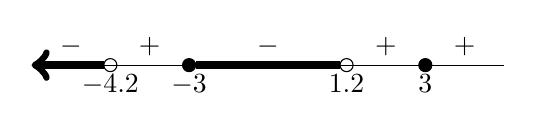
\begin{tikzpicture}
    \draw (0,0) -- (6,0);
    \node [circle,draw,scale=0.5] (a) at (1,0) {};
    \node [circle,draw,fill,scale=0.5] (b) at (2,0) {};
    \node [circle,draw,scale=0.5] (c) at (4,0) {};
    \node [circle,draw,fill,scale=0.5] (d) at (5,0) {};
    \node [below] at (a) {$-4.2$};
    \node [below] at (b) {$-3$};
    \node [below] at (c) {$1.2$};
    \node [below] at (d) {$3$};
    \node [above] at (0.5,0) {$-$};
    \node [above] at (1.5,0) {$+$};
    \node [above] at (3,0) {$-$};
    \node [above] at (4.5,0) {$+$};
    \node [above] at (5.5,0) {$+$};
    \draw [line width=1mm,<-] (0,0) to (a);
    \draw [line width=1mm] (b) to (c);
  \end{tikzpicture}

  Note that we do not change sign across the zero with the even multiplicity
  at $x=3$.

  $x\in(-\infty,\frac{-3-\sqrt{29}}{2})\cup[-3,\frac{-3+\sqrt{29}}{2})
    \cup\{3\}$

  Note that it turns out that $x=2$ is in an already rejected interval, so we
  don't need to make a hole for it.

  \bigskip

\item We want a circle whose diameter is the line segment between the points
$(5,4)$ and $(-3,-2)$. Using the distance and midpoint formulas:
\begin{enumerate}
\item{Determine the center of the circle.}

  The center of the circle will be at the midpoint of the two diameter points:

  $x=\frac{5-3}{2}=1$ and $y=\frac{4-2}{2}=1$

  $C(1,1)$
  
\item{Determine the radius of the circle.}

  The length of the radius can be calculated using the distance formula to find
  the distance between the center of the circle and one of its diameter points:

  $r=\sqrt{(1-5)^2+(1-4)^2}=\sqrt{(-4)^2+(-3)^2}=5$

  Just to check, let's calculate this using the other point:
  
  $r=\sqrt{(1+3)^2+(1+2)^2}=\sqrt{4^2+3^2}=5$

  As expected, we get the same answer.

  $r=5$

\item{What is the equation of the circle in standard form?}

  $(x-1)^2+(y-1)^2=25$
  
\item{What is the equation of the circle in general form?}

  $x^2-2x+1+y^2-2y+1=25$

  $x^2+y^2-2x-2y-23=0$
\end{enumerate}

\item Find the equation of the line containing the diameter in question (2):

  $m = \frac{4+2}{5+3}=\frac{6}{8}=\frac{3}{4}$
  
\begin{enumerate}
\item{In point/slope form.}

  $y-4=\frac{3}{4}(x-5)$ or $y+2=\frac{3}{4}(x+3)$

\item{In slope-intercept form.}

  $y-4=\frac{3}{4}x-\frac{15}{4}$

  $y=\frac{3}{4}x+\frac{1}{4}$
  
\item{In general form.}

  $\frac{3}{4}x-y+\frac{1}{4}=0$
  
\item{Find the equation of the line through the center of the circle and
  perpendicular to the line containing the stated diameter.}

  $m_{\perp}=-\frac{4}{3}$

  $y-1=-\frac{4}{3}(x-1)$

  Since I didn't ask for a particular form, you can leave it like this, or
  convert to y-intercept form:

  $y-1=-\frac{4}{3}x+\frac{4}{3}$

  $y=-\frac{4}{3}x+\frac{7}{3}$
\end{enumerate}

\item The amount of heat energy ($Q$) needed to change the temperature of an
object (without going through a phase change like melting or boiling) is jointly
proportional to the mass of the object ($m$) and the \emph{change} in
temperature ($\Delta T$).
\begin{enumerate}
\item Write an equation that models this physical phenomenon. Use $c$ for the
  constant of proportionality.
  \[Q=cm\D T\]
  
\item The MKS unit for heat energy is the Joule (J). The constant of
proportionality is specific to the substance being heated and is referred to as
the \emph{specific heat} of the substance. If $Q$ is measured in Joules ($J$),
$m$ is measured in grams ($g$), and temperature is measured in Kelvin (K), what
are the units of $c$?
\[J=\frac{J}{gK}gK\]
So the units of $c$ are $J/gK$.

\item In the lab, it is found that $41790J$ of heat energy raises the
temperature of $1L$ of water by $10K$. What is the specific heat of water?
(1L of water=1000g)

\[c=\frac{Q}{m\D T}=\frac{\SI{41790}{J}}{\SI{1000}{g}\cdot\SI{10}{K}}=
\SI{4.1790}{J/gK}\]
\end{enumerate}

\newpage

\item Consider the equation:
\[y=x^2+2x-5\]
For each of the parts below, use the graphing functions under the \emph{math}
(TI-89) or \emph{calc} (TI-83/84) menus to find the answer and submit a
screen-shot from your calculator that shows the correct answer.
\begin{enumerate}
\item Find the $y$-value when $x=1.3$ using the \emph{value} function.

  \includegraphics[scale=0.75]{hw6-5a.png}
  
\item Find the $x$-intercepts using the \emph{zero} function.

  \includegraphics[scale=0.75]{hw6-5b1.png}
  \includegraphics[scale=0.75]{hw6-5b2.png}

\item Determine the minimum value using the \emph{minimum} function.

  \includegraphics[scale=0.75]{hw6-5c.png}

  \newpage

\item Determine the $x$-values for $y=5$ using the \emph{intersect} function.
Note that you will need to add something to your graph to do this. Also note
that there are multiple answers.

  \includegraphics[scale=0.75]{hw6-5d1.png}
  \includegraphics[scale=0.75]{hw6-5d2.png}

\item Now graph the function $y=x^2+11$. Huh!? Nothing seems to appear! Why,
and how can you fix this? Submit a screen shot that uses your fix.

  \includegraphics[scale=0.75]{hw6-5e1.png}
  \includegraphics[scale=0.75]{hw6-5e2.png}
\end{enumerate}
\end{enumerate}

\end{document}
